\chapter{Arkitektur Worksheet}
Arkitekturen er opbygget af fire komponenter: \textit{manager}, \textit{moduler}, \textit{DB access} og \textit{DB}.
En skitse af arkitekturen kan ses på \cref{arkitektur_udkast_1}.
\begin{figure}[h]
	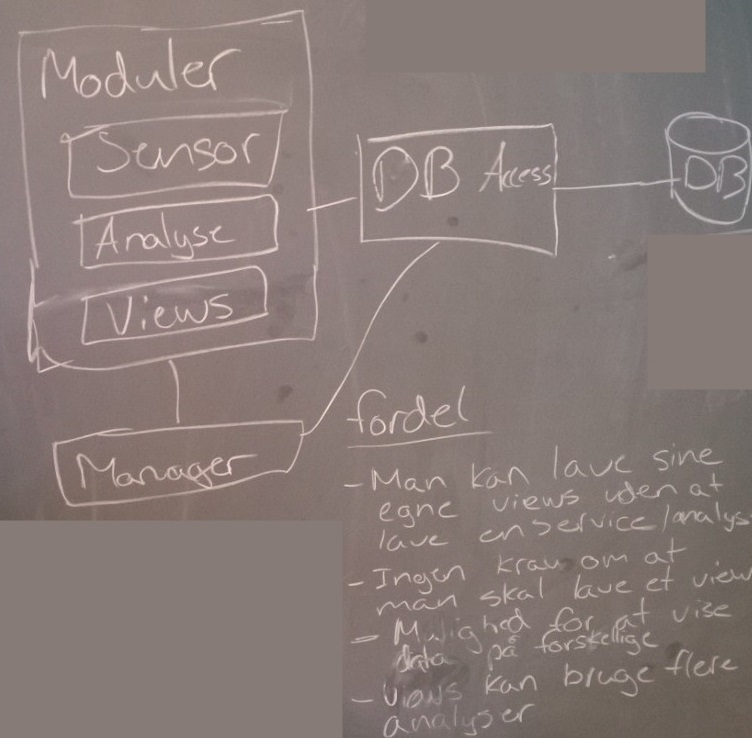
\includegraphics[width=\textwidth]{architecture_draft}
	\label{arkitektur_udkast_1}
	\caption{Første udkast til arkitektur.}
\end{figure}

\subsection*{Manager}
Denne komponent står for at holde styr på hvilke moduler der er installeret og opretter tabeller i databasen for dem.
\textit{Manageren} indeholder også et GUI så brugeren kan tilføje og fjerne moduler.
\textit{Manageren} har også logikken for hvilke \textit{analyse} moduler der kan vises i hvilke \textit{views}.
Desuden indeholder \textit{manageren} også et JSON skema for hver modul-type i \textit{moduler} komponenten.

\subsection*{Moduler}
Denne komponent består af tre lag: \textit{sensor}, \textit{analyse} og \textit{views}.
Alle moduler i hvert lag indeholder en JSON beskrivelse.

\paragraph{Sensor}
\textit{Sensor} laget indeholder alle de moduler der logger data fra sensor eller logger data fra applikationer.

\paragraph{Analyse}
\textit{Analyse} laget indeholder alle moduler der bruger et antal \textit{sensor} moduler og analyserer det data.
Dette modul foretager fx en del beregninger over tid og har et antal datatyper som output.

\paragraph{Views}
\textit{Views} laget indeholder alle moduler der gør det muligt at visualisere de analyserede data.
Den angiver hvilke og hvor mange datatyper den kan vise.

\subsection*{DB Access}
Denne komponent holder styr på hvem der skriver og læser fra databasen og på hvilken måde.

\subsection*{DB}
En sqlite database.

\section*{Arkitekturens styrker}
Denne modulbaserede arkitektur har \textit{moduler} komponenten som indeholder forskellige moduler.
Disse moduler kan kombineres og dette er en styrke i forhold til at man har mulighed for at tilføje flere moduler løbende.
Det giver en solid platform der giver mulighed for at udvikle flere moduler løbende.
\\
\\
Det giver mulighed for at et view kan bruges af mange analyser eller omvendt.
Da smartphones udvikler sig hele tiden og sikkert får en del nye sensorer i fremtiden er det ikke et problem, fordi det er muligt at tilføje et nyt sensor modul.

\textbf{Det har ikke været muligt at finde et umiddelbart arkitektur-mønster for dette.}